\documentclass{ctexart}
\usepackage{graphicx}
\usepackage{amsmath}
\usepackage{amsthm}
\usepackage{amssymb}
\usepackage{fancyhdr}
\usepackage{ifthen}
\usepackage{syntonly}
\usepackage[colorlinks, CJKbookmarks=true, linkcolor=red]{hyperref}
\pagestyle{plain}
\usepackage[raggedright]{titlesec}
\newtheorem{性质}{性质}
\newtheorem{定理}{定理}
\newtheorem{推论}{推论}
\begin{document}
\title{作业}
\author{计算机科学与技术系52班 杨定澄 \and 学号:2015011274 \and E-mail:892431401@qq.com}
\date{}
\maketitle
\section{生成数据}
rand.py用于产生数据,运行得到的A1,B1,C1,A2,B2,C2的数据存在对应名字的.txt里。

现已生成好。
\section{k-means}
kmeans.py实现了用k-means算法对D2进行聚类的结果,程序大约需花4秒左右。

聚类的结果如下:

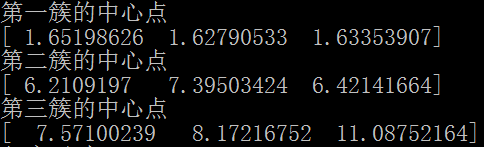
\includegraphics{1.png}

真实的情况是每组数据的中心点大约在$[1,1,1],[6,6,6],[7,8,9]$附近,可以看出结果比较稳合。
\section{MLE估计与分类正确率}
MLE.py用来估计参数与分类,程序要运行约6秒。

参数估计与分类结果如下:

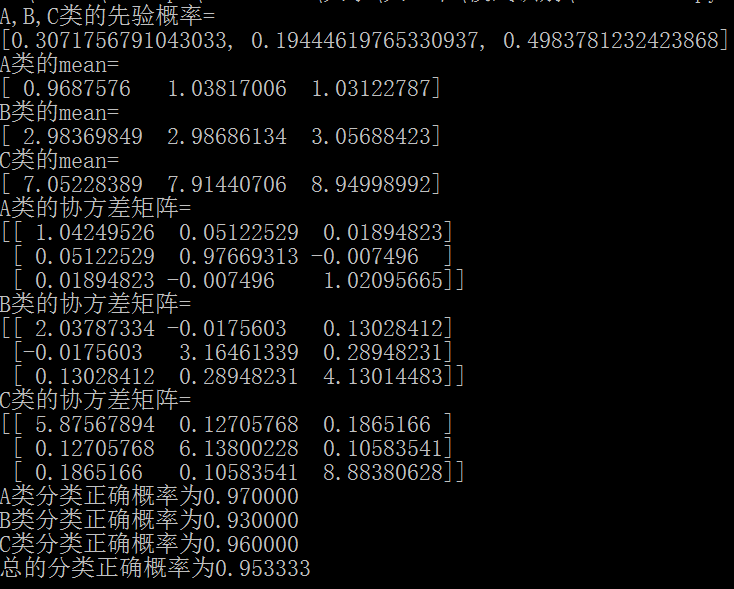
\includegraphics{2.png}

可以看到最后能有$95\%$的正确率,是相当不错的分类方法。

初始的$\mu$和协方差矩阵使用的是真实值,$P(\omega_i)$使用的是$\frac{1}{3}$,而更改成任意随机值后都会收敛至较优的解。(也可以通过调整迭代次数要结果更优,我这里是强制迭代30次)
\end{document}
